%%
%% This is file `sample-sigconf.tex',
%% adapted from the official ACM conference proceedings template.
%%
%% Canonical paper entry:
%% - body lives directly in this file
%% - bibliography lives in sample-base.bib
%%
\PassOptionsToPackage{hyphens}{url}
\PassOptionsToPackage{table}{xcolor}
\documentclass[sigconf,anonymous]{acmart}

\AtBeginDocument{%
  \providecommand\BibTeX{{%
    Bib\TeX}}}

%% Extra packages required by this paper body.
\usepackage{multirow}
\usepackage{bbm}
\usepackage{bm}
\usepackage{array}
\usepackage{diagbox}
\usepackage{bbding}
\usepackage{colortbl}
\usepackage{tabularx}
\usepackage{xspace}
\usepackage{pifont}
\usepackage{dblfloatfix}
\setlength{\emergencystretch}{0.6em}

\newcommand{\cmark}{\ding{51}}
\newcommand{\xmark}{\ding{55}}

\newcommand{\ie}{\textit{i.e.}\xspace}
\newcommand{\eg}{\textit{e.g.}\xspace}
\newcommand{\etc}{\textit{etc.}\xspace}
\newcommand{\Fref}[1]{\hyperref[#1]{Figure~\ref*{#1}}}
\newcommand{\Eref}[1]{\hyperref[#1]{Equation~(\ref*{#1})}}
\newcommand{\eref}[1]{\Eref{#1}}
\newcommand{\Tref}[1]{\hyperref[#1]{Table~\ref*{#1}}}
\newcommand{\Sref}[1]{\hyperref[#1]{Section~\ref*{#1}}}
\newcommand{\sref}[1]{\Sref{#1}}

\graphicspath{{figures/}}

%% Replace with official rights-form metadata when available.
\setcopyright{none}
\copyrightyear{2026}
\acmYear{2026}
\acmDOI{}
\acmConference[MM '26]{ACM Multimedia}{October 2026}{Anonymous Submission}
\acmISBN{}
\settopmatter{printacmref=false,printfolios=false}

\begin{document}

\title[CHORD]{CHORD: Calibrating Hallucinations via Object-Resonant Decoding in Multimodal Large Language Models}

% Double-blind submission: keep all author-identifying information disabled.
% \author{Kaiwen Deng}
% \email{dkw24@mails.tsinghua.edu.cn}
% \affiliation{%
%   \institution{Tsinghua Shenzhen International Graduate School, Tsinghua University}
%   \city{Shenzhen}
%   \country{China}}

% \author{Wenming Yang}
% \authornote{Corresponding author.}
% \email{yang.wenming@sz.tsinghua.edu.cn}
% \affiliation{%
%   \institution{Shenzhen International Graduate School \& Department of Electronic Engineering, Tsinghua University}
%   \city{Shenzhen}
%   \country{China}}

\renewcommand{\shortauthors}{Anonymous Submission}

\begin{abstract}
Multimodal Large Language Models remain text-native autoregressive systems: visual evidence conditions the hidden state, but token admission is still decided one step at a time. Hallucination therefore often emerges as a short-horizon decoding failure, where a locally plausible token enters the prefix before robust visual grounding is established. Existing training-free mitigation methods mainly penalize historical failures or rescore the current step, but they do not jointly test whether a candidate is supported by query-relevant visual regions and whether its immediate continuation remains visually grounded. In this paper, we propose \textbf{CHORD}, an inference-time framework for \emph{Calibrating Hallucinations via Object-Resonant Decoding}. CHORD evaluates candidate tokens with three coordinated signals: a past signal that preserves rollback-based protection against textual inertia, a current signal that measures query-conditioned visual support, and a future signal that probes short-horizon continuation through bounded rollout. To keep the method practical, CHORD performs anchor generation before autoregressive decoding and uses shared-KV batched rollout during candidate evaluation. Experiments on POPE, CHAIR, and MMBench with LLaVA-1.5 and InstructBLIP indicate two stable operating regimes: \textit{Past+Current} (\textit{CHORD-P+C}) delivers the strongest latency-efficient POPE gains, while Full CHORD yields the strongest overall quality metrics, including the largest CHAIR reduction while retaining the best MMBench accuracy across both backbones. These results indicate that multimodal decoding benefits from evaluating both \emph{support now} and \emph{stability next}.
\end{abstract}

\begin{CCSXML}
<ccs2012>
 <concept>
  <concept_id>10010147.10010257</concept_id>
  <concept_desc>Computing methodologies~Machine learning</concept_desc>
  <concept_significance>500</concept_significance>
 </concept>
 <concept>
  <concept_id>10010405.10010444</concept_id>
  <concept_desc>Applied computing~Computer vision</concept_desc>
  <concept_significance>300</concept_significance>
 </concept>
 <concept>
  <concept_id>10010147.10010178.10010179</concept_id>
  <concept_desc>Computing methodologies~Natural language processing</concept_desc>
  <concept_significance>300</concept_significance>
 </concept>
</ccs2012>
\end{CCSXML}

\ccsdesc[500]{Computing methodologies~Machine learning}
\ccsdesc[300]{Applied computing~Computer vision}
\ccsdesc[300]{Computing methodologies~Natural language processing}

\keywords{Hallucination Mitigation, Decode-Time Verification, Visual Grounding}

\maketitle

\section{Introduction}
\label{sec:intro}

\begin{figure}[t]
    \centering
    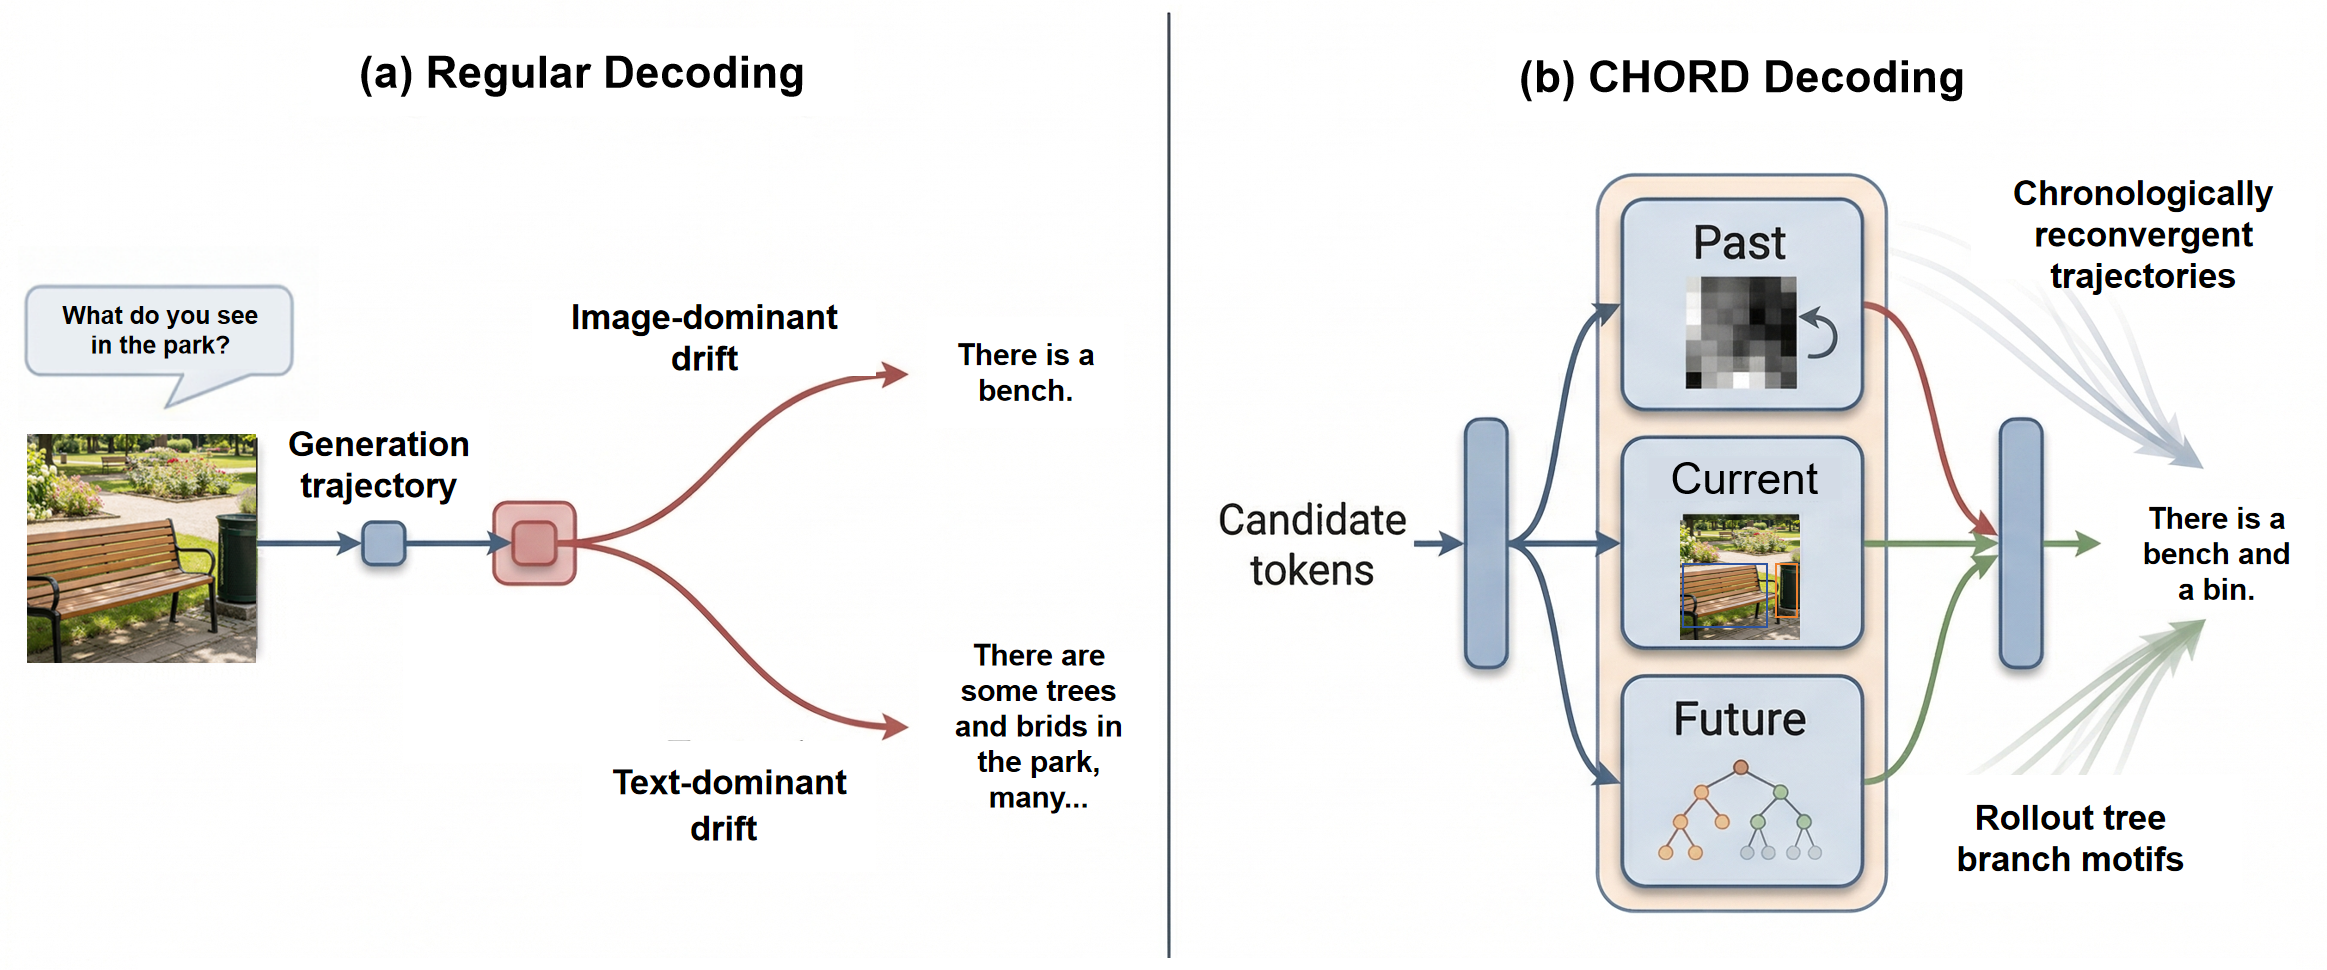
\includegraphics[width=\columnwidth]{figure1.png}
    \caption{CHORD reframes decode-time hallucination control as \emph{admission followed by short-horizon verification}. Left: regular decoding may admit a locally fluent but weakly grounded token and drift into text-dominated continuation. Right: CHORD screens the same admission through past rollback protection, current object resonance, and future rollout arbitration before commitment.}
    \Description{A two-part teaser figure for CHORD. The left half shows regular decoding drifting from a locally plausible token into text-dominated continuation. The right half shows CHORD evaluating candidate tokens through past, current, and future modules before selecting a grounded continuation.}
    \label{fig:teaser}
\end{figure}

Recent Multimodal Large Language Models (MLLMs)~\cite{alayrac2022flamingo,li2023blip2,liu2023improvedllava,instructblip,bai2024qwen2vl,chen2024internvl,ye2024mplugowl2,li2025llava_st} have substantially improved open-ended visual understanding and generation, but their outputs are still produced by text-native autoregressive decoding. Visual evidence conditions the hidden state, yet the final decision is still made one token at a time. This makes hallucination a decoding problem as much as a representation problem: once a visually weak token is admitted, subsequent tokens are generated from a prefix that already contains the error.

This failure manifests as multimodal hallucination~\cite{bai2025mllm_hallucination_survey,li2023pope,rohrbach2018object,lovenia2023nope,wang2023amber,wu2024relationship_hallucinations,jing2023faithscore}: the model mentions unsupported objects, attributes, or relations while remaining linguistically smooth. The problem is especially acute in trust-sensitive applications because the generated text sounds coherent even when it is poorly grounded.

Existing mitigation strategies attack the problem at different stages. Training-time approaches improve factuality through additional supervision, preference optimization, or revision-aware alignment~\cite{liu2023aligning,chen2024hio,zhang2024reflective_instruction,lee2024volcano,yu2024rlhfv,sun2023llava_rlhf,peng2025sentinel}, but they require retraining and model-specific adaptation. Post-hoc correction and detection pipelines~\cite{yin2023woodpecker,gunjal2024detecting_preventing,zhang2025dhcp,jing2023faithscore} intervene only after an unstable continuation has already been produced or must be diagnosed separately. Decode-time intervention is therefore attractive because it is training-free and acts at token admission. However, most existing decode-time baselines remain predominantly local: they rely on contrastive or grounded logits~\cite{leng2023mitigating,favero2024m3id,deng2024clipguided,wang2024icd,chuang2023dola,jiang2024hacl,kim2024code}, retrospective attention tests~\cite{huang2024opera_cvpr,woo2024ritual,liu2024paying_attention_image,xu2025tarac,kai2024sh2}, or self-feedback loops~\cite{zhang2025degf,cao2025cofidec}, but they do not explicitly test whether an admitted token stays grounded over the next few decoding steps.

We describe this failure mode as \textbf{structural temporal collapse}: a locally acceptable token can still push the decoder into a short-horizon regime in which image-linked attention weakens and textual self-conditioning takes over. This is an operational description, not a claim of formal causality. The key implication is practical: local plausibility is not enough. A token should be judged by both the evidence it currently receives and the continuation tendency it induces.

To address this gap, we propose \textbf{CHORD}, a training-free decoding framework for \emph{admission-time verification}. CHORD combines three signals: rollback-based protection against already-collapsed prefixes, current support from relevant visual regions, and a short future rollout that tests whether continuation remains grounded. The current term answers ``is this token visually supported now?''; the future term answers ``does this token keep the branch grounded next?'' Unlike rollback-only methods, CHORD does not wait for collapse to become visible in the prefix; unlike current-step contrastive rules or generic lookahead, it tests whether a candidate is grounded \emph{now} and stable \emph{next}.

Because future arbitration introduces additional test-time compute, CHORD also includes practical execution rules: anchor generation is performed once before autoregressive decoding, branch evaluation reuses shared prefix KV-cache, and unstable branches are terminated early. The resulting method is closer to bounded test-time verification than to unrestricted search, which is why we frame it as a decode-time control rule rather than a global search procedure. The core question is therefore not only whether text is fluent, but whether token admission remains faithful to visual evidence under practical latency constraints.

Our contributions are summarized as follows:
\begin{itemize}
    \item We formulate decode-time hallucination control as a \emph{trajectory verification} problem and characterize a practical failure mode, \emph{structural temporal collapse}, in which a weakly grounded admission induces text-dominated continuation.
    \item We propose CHORD, a training-free admission verifier that combines OPERA-compatible rollback protection, late-layer object-resonant current scoring, and bounded future arbitration in a single reranking rule.
    \item We operationalize a late-layer decoder-to-vision signal by aggregating the last four decoder blocks and show how shared-KV rollout makes short-horizon branch verification practical at inference time.
    \item We evaluate CHORD on POPE, CHAIR, and MMBench across LLaVA-1.5 (7B) and InstructBLIP (7B), showing a reproducible two-regime trade-off: \textit{Past+Current} gives the strongest latency-efficient discriminative gains, while Full CHORD gives the strongest overall quality metrics and retained MMBench accuracy.
\end{itemize}

\section{Related Work}
\label{sec:related_work}

\subsection{MLLM Hallucination}

Modern MLLMs~\cite{alayrac2022flamingo,li2023blip2,liu2023improvedllava,instructblip,bai2023qwen,wang2023cogvlm,zhu2023minigpt,chen2024internvl,ye2024mplugowl2} align image representations with pretrained language models, enabling strong zero-shot and instruction-following performance. Nevertheless, hallucination remains a persistent issue~\cite{bai2025mllm_hallucination_survey,zhou2023analyzing,li2023pope,rohrbach2018object,lovenia2023nope,wang2023amber,guan2024hallusionbench,wu2024relationship_hallucinations,lu2023agnosia}. Prior analyses attribute these failures to language-prior dominance, weak grounding, and instability in long-form autoregressive generation. Our work focuses on the decode-time aspect of this problem.

\subsection{Training-Time and Post-Hoc Mitigation}

One line of work improves grounding during training through instruction tuning, preference optimization, hallucination-aware objectives, or feedback-guided revision~\cite{liu2023aligning,chen2024hio,zhang2024reflective_instruction,lee2024volcano,yu2024rlhfv,sun2023llava_rlhf,peng2025sentinel}. These methods can be effective, but they require additional supervision and model adaptation. Another line of work introduces post-hoc correction modules, verifiers, or hallucination detectors~\cite{yin2023woodpecker,gunjal2024detecting_preventing,zhang2025dhcp,jing2023faithscore}. Such approaches improve factuality after generation, but they increase system complexity and latency.

\subsection{Decode-Time Intervention and Lookahead}

Training-free decode-time methods are especially relevant to our setting. Contrastive and grounded decoding suppress unsupported continuations by comparing logits or injecting auxiliary visual evidence~\cite{leng2023mitigating,favero2024m3id,deng2024clipguided,wang2024icd,chuang2023dola,jiang2024hacl,kim2024code}. Attention-based methods use internal dynamics to penalize textual over-reliance or trigger rollback, including OPERA~\cite{huang2024opera_cvpr}, RITUAL~\cite{woo2024ritual}, TARAC~\cite{xu2025tarac}, SH2~\cite{kai2024sh2}, and attention-guided reweighting~\cite{liu2024paying_attention_image}. Self-feedback methods further ask the model to verify its own generations through synthetic evidence or iterative revision~\cite{zhang2025degf,cao2025cofidec}. In parallel, recent work on test-time compute scaling and lookahead decoding suggests that short-horizon forecasting can improve model decisions~\cite{fu2024lookahead,gagrani2024speculative_mllm,gao2024cantor,cheng2025think_more}. CHORD combines these directions with a narrower objective than generic search: it uses query-relevant visual support to judge whether a token should enter the prefix, then uses a bounded future rollout to test whether that admission remains visually stable over the next few steps.

\section{Methodology}
\label{sec:Methodology}

We introduce \textbf{CHORD}, a training-free decoding framework for reducing hallucination in MLLMs. At each decoding step, CHORD does not immediately accept the highest-logit token. Instead, it reranks a small candidate set using three signals: a \emph{past} signal for historical protection, a \emph{current} signal for object-resonant grounding, and a \emph{future} signal for short-horizon rollout evaluation. The distinctive design choice is to pair \emph{support now} with \emph{stability next}: CHORD does not merely ask whether a candidate looks plausible at the current step, but whether admitting it is likely to preserve grounding over the next few decoding steps.

\begin{figure*}[t]
    \centering
    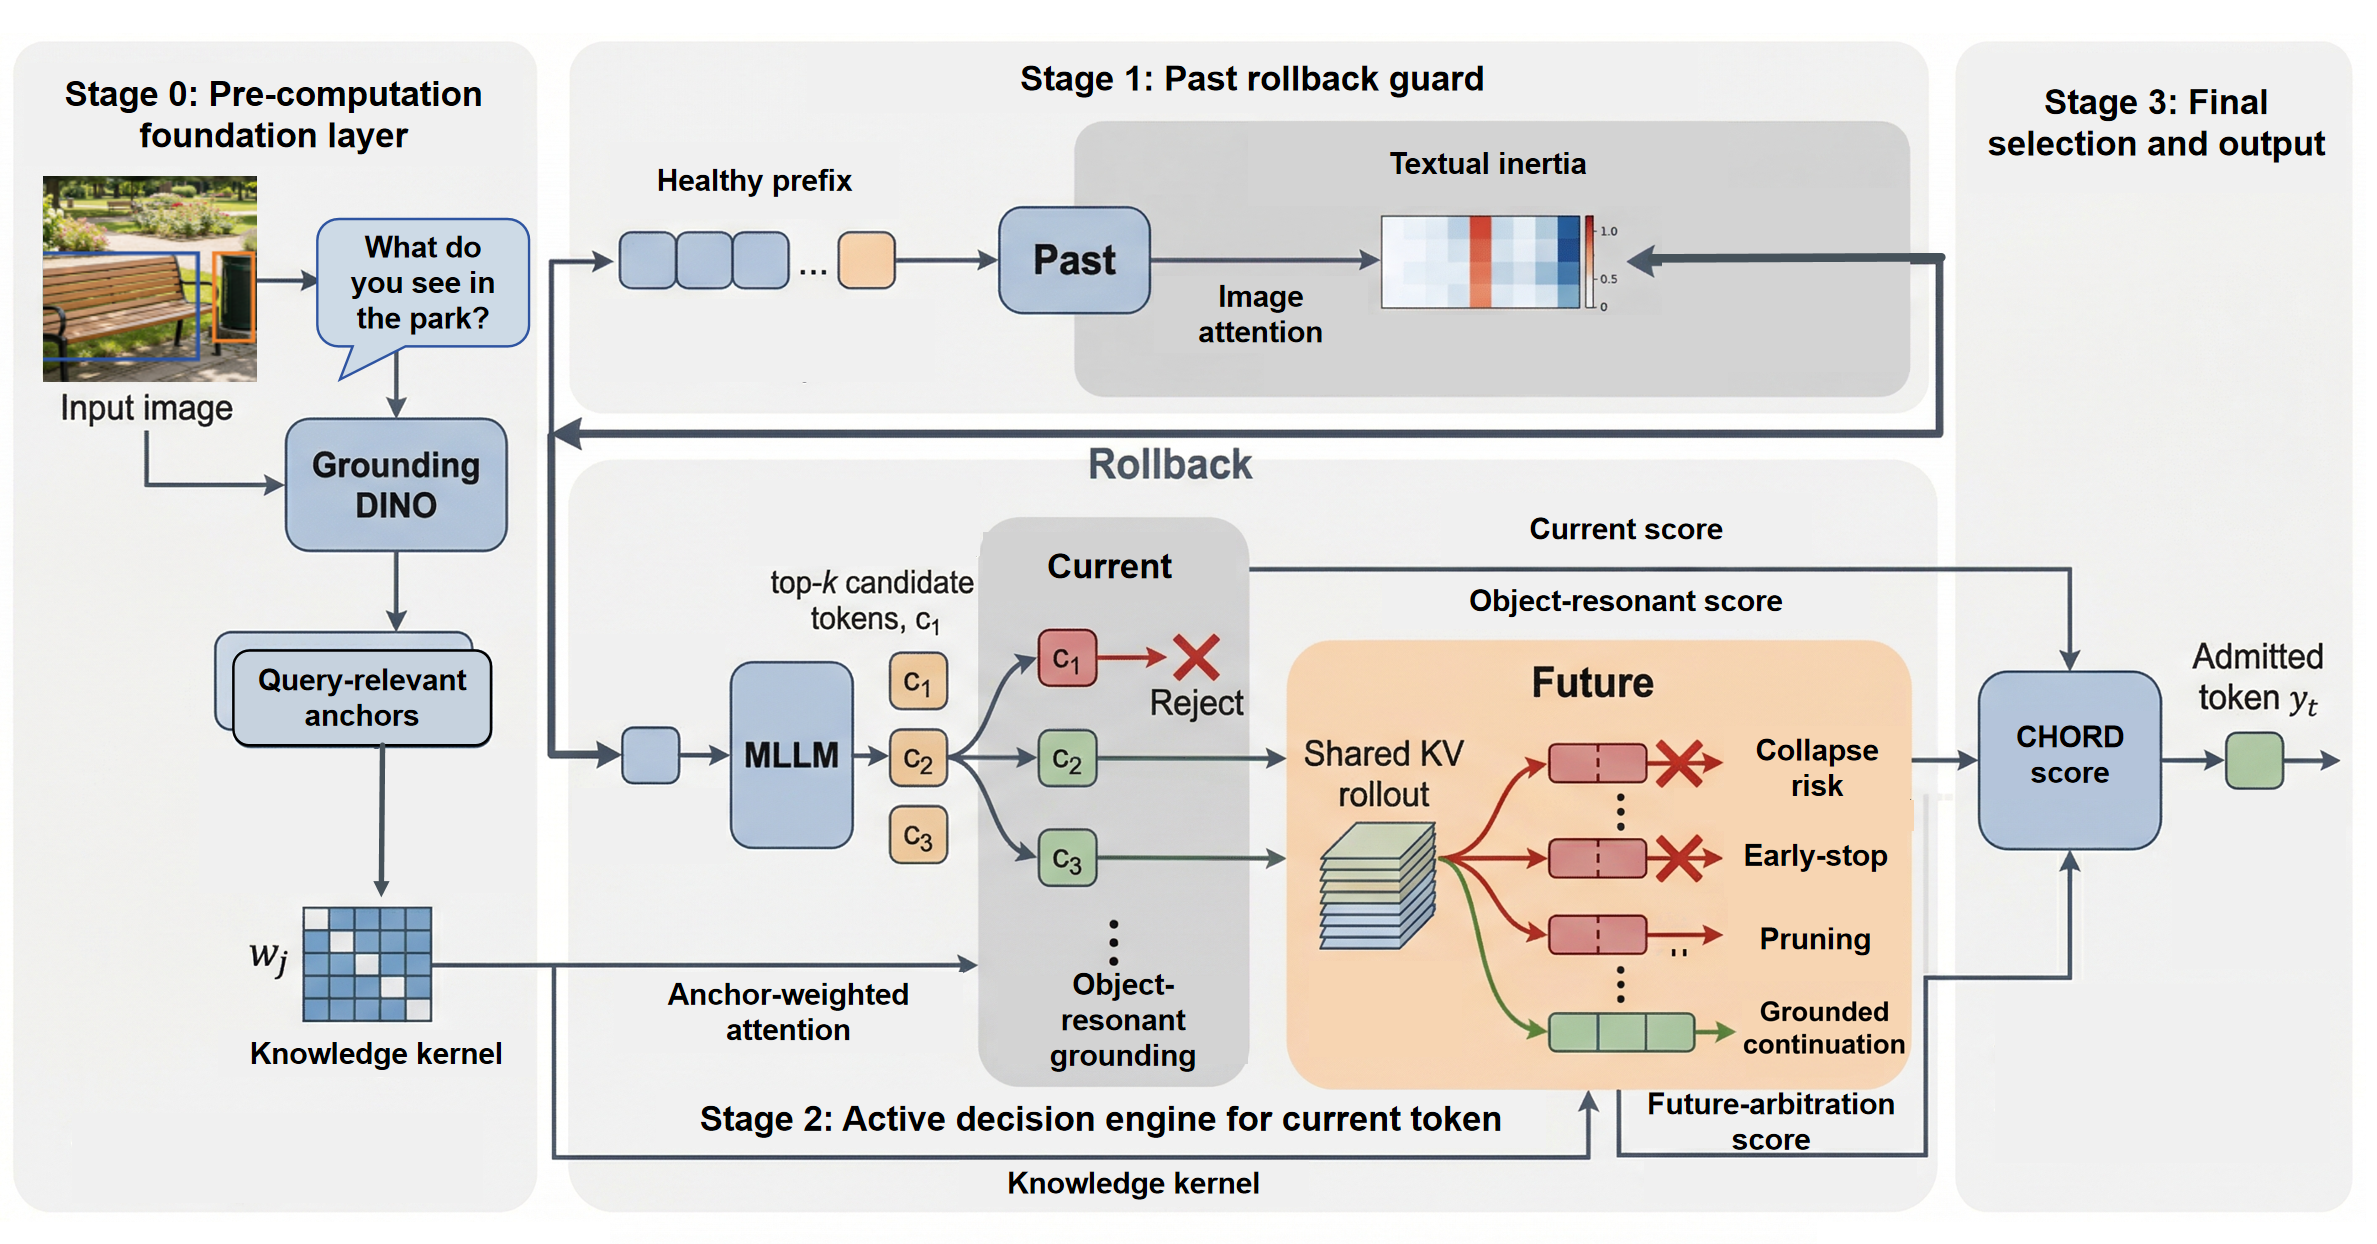
\includegraphics[width=\textwidth]{figure2.png}
    \caption{Method overview of CHORD. Stage 0 constructs query-relevant anchors and anchor weights before autoregressive decoding. Stage 1 applies rollback-based past protection to repair already-collapsed prefixes. Stage 2 reranks the top-$k$ candidates through object-resonant current scoring and bounded future arbitration under shared-KV rollout. Stage 3 admits the candidate with the highest aggregate score.}
    \Description{A four-stage method figure for CHORD. The left side shows image and query input, Grounding DINO proposals, and anchor weights. The middle upper path shows the past rollback guard. The middle lower path shows top-k candidates scored by current object resonance and future rollout arbitration. The right side shows final score aggregation and token admission.}
    \label{fig:method_overview}
\end{figure*}

\noindent\textbf{Problem Setting.} Let a pretrained MLLM parameterized by $\theta$ receive a visual input $v$ and a textual query $x$. The visual encoder maps $v$ to visual tokens $\mathcal{V}=\{v_1,\dots,v_N\}$. At decoding step $t$, the decoder defines
\begin{equation}
    p_\theta(y_t \mid \mathcal{V}, x, y_{<t}) = \text{Softmax}\!\left(f_\theta(y_t \mid \mathcal{V}, x, y_{<t})\right),
\end{equation}
where $y_{<t}$ is the current prefix and $f_\theta$ denotes the pre-softmax logits. CHORD first applies the same retrospective rollback test as OPERA to the prefix. If the test is triggered, the prefix is repaired and the current step is recomputed on the repaired state $\tilde{y}_{<t}$. CHORD then forms the candidate set
\begin{equation}
    \mathcal{C}_t = \operatorname{TopK}\!\left(p_\theta(\cdot \mid \mathcal{V}, x, \tilde{y}_{<t}), k\right),
\end{equation}
and reranks candidates before admission.

\subsection{Candidate Scoring}
\label{sec:astar}

After rollback handling, CHORD evaluates each candidate token $y_t^{(c)} \in \mathcal{C}_t$ with
\begin{equation}
    S_{\mathrm{CHORD}}(y_t^{(c)}) = S_{\mathrm{past}}(y_t^{(c)}) + \lambda_{\mathrm{cur}} V_{\mathrm{res}}(y_t^{(c)}) + \lambda_{\mathrm{fut}} F_{\mathrm{harm}}(y_t^{(c)}),
\end{equation}
and outputs the candidate with the highest final score over the surviving set. This rule is a bounded reranking objective rather than a global sequence-search objective.

\noindent\textbf{Past: rollback-based historical protection.} We reuse the retrospective safeguard of OPERA~\cite{huang2024opera_cvpr} to detect severe columnar attention concentration on previously generated text. This component operates on the prefix before candidate reranking. Once the step is re-entered on a valid prefix $\tilde{y}_{<t}$, the past score for each candidate is the local log-probability
\begin{equation}
    S_{\mathrm{past}}(y_t^{(c)}) = \log p_\theta(y_t^{(c)} \mid \mathcal{V}, x, \tilde{y}_{<t}),
\end{equation}
which preserves compatibility with the underlying decoder whenever rollback is inactive.

\noindent\textbf{Late-layer attention aggregation.} Both the current and future terms use decoder attention to visual and textual source positions. Let $a_{\ell,h}(q \rightarrow z)$ denote the attention from query token $q$ to source token $z$ at decoder layer $\ell$ and head $h$. We first average over heads within each block,
\begin{equation}
    \bar{a}_{\ell}(q \rightarrow z) = \frac{1}{H}\sum_{h=1}^{H} a_{\ell,h}(q \rightarrow z),
\end{equation}
then aggregate only the last four decoder blocks,
\begin{equation}
    \begin{aligned}
        \mathcal{L}_{\mathrm{late}} &= \{L_{\mathrm{dec}}-3,\ldots,L_{\mathrm{dec}}\}, \\
        A_t(q \rightarrow z)
        &=
        \frac{\sum_{\ell \in \mathcal{L}_{\mathrm{late}}} \bar{a}_{\ell}(q \rightarrow z)}
        {\sum_{z' \in \mathcal{S}_t}\sum_{\ell \in \mathcal{L}_{\mathrm{late}}}
        \bar{a}_{\ell}(q \rightarrow z')}.
    \end{aligned}
\end{equation}
where $\mathcal{S}_t$ contains the monitored source positions at step $t$: visual tokens, the textual query, and prefix tokens, while excluding structural separator positions. We use the last four decoder blocks as an empirically chosen late-layer operating window: mid-stack attention is often too diffuse, whereas the final block alone is more brittle and sensitive to the immediately preceding token. \Fref{fig:design_evidence} visualizes this choice and supports the stability-specificity trade-off that motivated it.

\noindent\textbf{Current: object-resonant visual support.} To bias candidate selection toward query-relevant image evidence, CHORD builds a lightweight object set once before autoregressive decoding. An external region proposer such as Grounding DINO~\cite{liu2023groundingdino} is queried with the textual prompt $x$, yielding anchors $\mathcal{B}=\{b_i\}$ together with confidence scores. We retain the top proposals after confidence thresholding. Each anchor is assigned a relevance weight $r_i \in [0,1]$ from the text-conditioned detector score, and each visual token receives
\begin{equation}
    w_j = 1 + \alpha \max_i \left(\mathbbm{1}(v_j \in b_i)\, r_i\, s_i\right),
\end{equation}
where $s_i$ denotes proposal confidence and $\mathbbm{1}(v_j \in b_i)$ indicates that visual token $v_j$ falls inside anchor $b_i$. For each candidate branch, CHORD temporarily appends $y_t^{(c)}$ to $\tilde{y}_{<t}$ and performs one forward pass conditioned on that candidate. The current object-resonant score is then
\begin{equation}
    V_{\mathrm{res}}(y_t^{(c)}) = \sum_{j=1}^{N} w_j\, A_t(y_t^{(c)} \rightarrow v_j).
\end{equation}
This candidate-conditioned pass is reused as the initial state of future rollout for the same branch. Hence, $V_{\mathrm{res}}$ measures \emph{support now}, not merely generic decoder preference.

\noindent\textbf{Why current and future signals are complementary.} The current signal and the future signal address different failure modes. A purely current-step rule can still overvalue a candidate that briefly attends to a relevant object but immediately hands control back to the textual prefix after admission. Conversely, a purely future-oriented rule can become unnecessarily conservative when multiple candidates have similar short-horizon continuation but only one is directly supported by query-relevant regions at the admission step. CHORD therefore separates \emph{admission support} from \emph{continuation stability}. The current score acts as an object-conditioned local filter that favors candidates already aligned with query-relevant evidence, while the future score asks whether that local alignment persists over the next few decoding steps. In this sense, the two signals are not redundant: $V_{\mathrm{res}}$ checks whether the candidate is visually plausible \emph{now}, whereas $F_{\mathrm{harm}}$ checks whether accepting it is likely to keep the trajectory visually grounded \emph{after} admission.

\subsection{Future Rollout and Harmonic Arbitration}
\label{sec:oracle}

The central idea of CHORD is to evaluate not only the current candidate, but also the immediate continuation it induces. Starting from the candidate-conditioned state above, CHORD greedily rolls each surviving branch forward for a short horizon $m$. At rollout step $\tau \in \{1,\dots,m\}$, we measure the weighted visual attention mass
\begin{equation}
    V_\tau(y_t^{(c)}) = \sum_{j=1}^{N} w_j\, A_{t+\tau}(y_{t+\tau} \rightarrow v_j),
\end{equation}
and the textual attention mass
\begin{equation}
    T_\tau(y_t^{(c)}) = \sum_{q=0}^{t+\tau-1} A_{t+\tau}(y_{t+\tau} \rightarrow y_q).
\end{equation}
Under the normalization above, $V_\tau$ and $T_\tau$ cover the monitored visual and textual mass used by CHORD. We define the stepwise branch utility
\begin{equation}
    R_\tau(y_t^{(c)}) = V_\tau(y_t^{(c)}) - \lambda_{\mathrm{txt}} T_\tau(y_t^{(c)}),
\end{equation}
and accumulate it until the branch terminates:
\begin{equation}
    \tau^\star(y_t^{(c)}) = \min \Bigl(m,\ \min \{\tau \mid \rho_\tau(y_t^{(c)}) < \tau_{\mathrm{abort}}\}\Bigr),
\end{equation}
\begin{equation}
    F_{\mathrm{harm}}(y_t^{(c)}) = \sum_{\tau=1}^{\tau^\star(y_t^{(c)})} R_\tau(y_t^{(c)}),
\end{equation}
where $\tau^\star$ is either the full rollout horizon or the first abort point triggered by low visual ratio. In the default quality setting used for the main tables, $\tau_{\mathrm{abort}}=0$, so future scoring uses the full short horizon; in the latency study, nonzero $\tau_{\mathrm{abort}}$ enables early stopping to avoid spending rollout compute on branches that have already become text-dominated. This future term therefore favors branches whose short-horizon continuations remain visually anchored while naturally shortening clearly unstable ones. We call this bounded rollout test \emph{harmonic temporal arbitration}.

\subsection{Efficient Rollout Execution}
\label{sec:bb}

Naively evaluating $k$ candidates for $m$ future steps introduces $\mathcal{O}(k \times m)$ extra decoding work. CHORD reduces this cost with two simple optimizations.

\noindent\textbf{Shared-KV batched rollout.} All candidates share the same historical prefix. We therefore reuse the prefix KV-cache and batch the $k$ candidate branches together, so candidate-conditioned evaluation and subsequent rollout are implemented as parallel forward passes rather than $k$ independent runs. The first batched branch expansion supplies the attention needed for $V_{\mathrm{res}}$, while the cached branch states are reused for the remaining rollout steps.

\noindent\textbf{Early rejection and stopping.} CHORD prunes branches in two stages:
\begin{enumerate}
    \item \textit{Current-step rejection.} After the candidate-conditioned forward pass, any branch with $V_{\mathrm{res}}(y_t^{(c)}) < \epsilon$ is discarded immediately. The surviving set is
    \begin{equation}
        \mathcal{C}^{\mathrm{keep}}_t = \left\{y_t^{(c)} \in \mathcal{C}_t \mid V_{\mathrm{res}}(y_t^{(c)}) \ge \epsilon \right\}.
    \end{equation}
    In our default setting, $\epsilon=0$, so only candidates with zero current support are removed at this stage.
    \item \textit{Future-step early stopping.} During rollout, if the visual ratio
    \begin{equation}
        \rho_\tau(y_t^{(c)}) = \frac{V_\tau(y_t^{(c)})}{V_\tau(y_t^{(c)}) + T_\tau(y_t^{(c)})}
    \end{equation}
    falls below the abort threshold $\tau_{\mathrm{abort}}$, the branch terminates at $\tau^\star(y_t^{(c)})$ and receives the truncated score in Eq.~(13). This avoids spending the full horizon on candidates that already exhibit unstable continuation.
\end{enumerate}

The final admission rule is therefore
\begin{equation}
    \hat{y}_t = \arg\max_{y_t^{(c)} \in \mathcal{C}^{\mathrm{keep}}_t} S_{\mathrm{CHORD}}(y_t^{(c)}).
\end{equation}
These execution rules preserve the benefit of short-horizon forecasting while keeping CHORD within the efficiency range of practical decode-time intervention.

\subsection{Complexity and Practical Behavior}
\label{sec:complexity}

Relative to greedy decoding, CHORD adds two forms of test-time work: candidate-conditioned scoring and short-horizon branch rollout. If each step keeps $k$ candidates and rolls each surviving branch forward for $m$ steps, naive evaluation would require up to $\mathcal{O}(k(1+m))$ branch-state expansions per decoding step in addition to the base forward pass. The main practical concern is therefore not asymptotic complexity alone, but whether these extra expansions can be executed without recomputing the shared prefix.

CHORD reduces this cost in two ways. First, all branches inherit the same historical prefix, so the prefix KV-cache is computed once and then reused across candidate-conditioned passes and subsequent rollout steps. The actual extra cost is thus dominated by incremental branch extensions rather than full-sequence recomputation. Second, the effective branch count is usually smaller than $k$: after the current-step resonance check, only candidates with nonzero current support are retained, and future-step aborting further shortens trajectories that have already become text-dominated. Denoting the average number of surviving branches by $k' \le k$ and the average realized rollout depth by $\bar{m} \le m$, the practical extra cost is better viewed as $\mathcal{O}(k' \bar{m})$ rather than the worst-case bound.

This perspective is important for interpreting the later experiments. CHORD should not be understood as an unrestricted tree search that attempts to optimize an entire sequence globally. Instead, it is a bounded decode-time control rule that selectively spends additional compute only on locally ambiguous admissions. The resulting behavior is closer to \emph{adaptive test-time verification} than to exhaustive search, which is why the method can still remain competitive in latency-sensitive settings.

\subsection{Design Discussion}

CHORD is built around three design choices. First, it uses a late-layer attention window rather than full-stack aggregation: earlier blocks are often too diffuse for reliable token admission, while the final block alone is brittle; the last-four-block aggregate was selected as a practical trade-off rather than claimed as a universal optimum. Second, it keeps current support and future arbitration separate, because ``supported now'' and ``stable next'' are related but distinct questions. Third, it uses bounded rollout rather than unrestricted search: the goal is to detect risky admissions before they enter the prefix, not to globally optimize the entire continuation. These choices make CHORD diagnostic rather than exhaustive, and keep the added test-time cost interpretable.

\section{Experiments}
\label{sec:experiments}

We evaluate CHORD on both hallucination-focused benchmarks and broader multimodal benchmarks. The experimental section is organized around three questions: (1) do object-resonant and future-aware candidate evaluations reduce hallucination, (2) what latency cost does rollout introduce and how much do our optimizations recover, and (3) can CHORD improve grounding without imposing a strong alignment tax on broader multimodal ability?

\subsection{Experimental Settings}

\noindent\textbf{Models.} We test CHORD on two open-source MLLMs: LLaVA-1.5 (7B)~\cite{liu2023improvedllava} and InstructBLIP (7B)~\cite{instructblip}. They cover distinct alignment recipes and visual backbones. CHORD is plugged into the released checkpoints without any parameter updates.

\noindent\textbf{Benchmarks.} We follow prior decode-time hallucination studies~\cite{huang2024opera_cvpr,leng2023mitigating} and use three public benchmarks.
POPE~\cite{li2023pope} evaluates object hallucination with binary questions over the Random, Popular, and Adversarial splits.
CHAIR~\cite{rohrbach2018object} measures hallucination in free-form captioning on MSCOCO, with sentence-level ($\text{CHAIR}_S$) and image-level ($\text{CHAIR}_I$) ratios.
MMBench~\cite{liu2023mmbench} is used as a broad-spectrum retention check for general multimodal reasoning. Together, these benchmarks cover both discriminative and open-ended settings.

\noindent\textbf{Baselines.} Our main-paper tables report Greedy Decoding together with representative decode-time baselines from the three closest families: DoLa~\cite{chuang2023dola} for layer-contrast decoding, VCD~\cite{leng2023mitigating} for visual contrastive decoding, and OPERA~\cite{huang2024opera_cvpr} for rollback-based intervention. We also checked Nucleus Sampling and HALC~\cite{chen2024halc} in the same evaluation pipeline, but keep the main-paper tables focused on the nearest inference-time comparators rather than exhaustively listing every variant. We discuss training-time methods in Related Work, but do not treat them as direct main-table baselines because they operate under different supervision and adaptation budgets. OPERA remains the closest prior because CHORD inherits its retrospective safeguard while adding object-resonant current scoring and bounded future verification.

\noindent\textbf{Implementation Details.} Unless otherwise stated, CHORD uses top-$k$ candidate reranking with $k=5$ and a rollout horizon of $m=3$. For the current and future terms, we set $\alpha=0.5$, $\lambda_{\mathrm{cur}}=0.25$, $\lambda_{\mathrm{fut}}=0.05$, and $\lambda_{\mathrm{txt}}=1.0$. Grounding DINO~\cite{liu2023groundingdino} provides query-conditioned anchor proposals with box and text thresholds of $0.25$ and $0.2$, respectively, and we retain at most $8$ proposals per example after thresholding. The proposer is invoked once before autoregressive decoding and the retained proposals are cached for the full generation process, so the decode-time rule does not repeatedly call the detector at each step. Accordingly, CHORD can be interpreted as a guidance-based decoding framework that couples the base MLLM with lightweight external perception at admission time. All attention-derived quantities use the layer-aggregated decoder-to-vision signal from the last four decoder blocks, which was the most reliable late-stage window for stable object localization in our preliminary analysis. We use $\epsilon=0$ for current-step rejection. For the main quality tables, we set $\tau_{\mathrm{abort}}=0$ so that future scoring uses the full short horizon; for the latency analysis, we additionally sweep nonzero $\tau_{\mathrm{abort}}$ settings to quantify the value of early stopping. Across POPE, CHAIR, and MMBench we keep prompts, answer parsing, and benchmark-side evaluation scripts fixed; only the decode-time decision rule changes. We therefore interpret MMBench primarily as a retention check on broader multimodal ability rather than as the paper's primary optimization target. ITL is reported as average per-token decoding latency under this fixed proposal policy on a single NVIDIA A100 GPU.

\subsection{Main Results on Hallucination Mitigation}

\noindent\textbf{Two operating points emerge.} The results do not suggest that a single CHORD configuration dominates every metric. Instead, they indicate two stable operating points. \textit{Past+Current} (\textit{CHORD-P+C}) is the strongest latency-efficient setting on POPE, whereas Full CHORD is the stronger configuration for open-ended sentence-level hallucination reduction. This division matches the roles of the two added signals: the current term primarily improves admission quality, whereas the future term is most beneficial when one weak admission can influence a longer continuation.

\begin{table*}[t]
\centering
\scriptsize
\setlength{\tabcolsep}{4pt}
\caption{Main quantitative comparison. We report the full CHORD configuration against external decode-time baselines. For each model we report average POPE F1 across the three splits, POPE Adversarial F1, CHAIR sentence/image hallucination ratios, MMBench accuracy, and per-token inference latency (ITL, ms/token). Lower ($\downarrow$) CHAIR and ITL are better; higher ($\uparrow$) POPE/MMBench are better. Bold indicates the best result in each column. Internal CHORD operating points are analyzed separately in \Tref{tab:family_tradeoff} and \Tref{tab:operating_points}.}
\label{tab:main_results}
\begin{tabular}{l|cccccc|cccccc}
\toprule
\multicolumn{1}{c|}{} & \multicolumn{6}{c|}{\textbf{LLaVA-v1.5-7B}} & \multicolumn{6}{c}{\textbf{InstructBLIP-7B}} \\
\cmidrule(lr){2-7} \cmidrule(lr){8-13}
\textbf{Method} & Avg. F1 $\uparrow$ & Adv. F1 $\uparrow$ & CH$_S$ $\downarrow$ & CH$_I$ $\downarrow$ & MMBench $\uparrow$ & ITL $\downarrow$ & Avg. F1 $\uparrow$ & Adv. F1 $\uparrow$ & CH$_S$ $\downarrow$ & CH$_I$ $\downarrow$ & MMBench $\uparrow$ & ITL $\downarrow$ \\
\midrule
Greedy          
& 0.8488 & 0.8036 & 0.2291 & 0.2046 & 68.63 & \textbf{19.73} 
& 0.8659 & 0.8327 & 0.2140 & 0.3380 & 69.34 & \textbf{16.47} \\
OPERA~\cite{huang2024opera_cvpr} 
& 0.8483 & 0.8042 & 0.2284 & 0.1996 & 68.65 & 21.69 
& 0.8577 & 0.8327 & 0.2180 & 0.3320 & 69.27 & 16.90 \\
VCD~\cite{leng2023mitigating}   
& 0.8403 & 0.8031 & 0.2183 & 0.2061 & 68.29 & 33.07 
& 0.8428 & 0.8173 & 0.2060 & 0.3480 & 68.70 & 24.80 \\
DoLa~\cite{chuang2023dola}      
& 0.8502 & 0.8103 & 0.3276 & 0.3517 & 68.63 & 23.11 
& 0.8488 & 0.8408 & 0.3090 & 0.4260 & 69.41 & 19.03 \\
\textbf{CHORD}                  
& \textbf{0.8752} & \textbf{0.8453} & \textbf{0.1548} & \textbf{0.1754} & \textbf{69.78} & 37.31 
& \textbf{0.8924} & \textbf{0.8651} & \textbf{0.1347} & \textbf{0.2795} & \textbf{70.82} & 35.86 \\
\bottomrule
\end{tabular}
\end{table*}

\Tref{tab:main_results} centers the external comparison on the full CHORD configuration. On LLaVA-1.5, CHORD raises Avg.\ F1 from $0.8488$ to $0.8752$ and Adv.\ F1 from $0.8036$ to $0.8453$, while reducing $\text{CHAIR}_S$ from $0.2291$ to $0.1548$ and $\text{CHAIR}_I$ from $0.2046$ to $0.1754$. On InstructBLIP, the same pattern remains visible: CHORD improves Avg.\ F1 from $0.8659$ to $0.8924$, lifts Adv.\ F1 from $0.8327$ to $0.8651$, reduces $\text{CHAIR}_S$ from $0.2140$ to $0.1347$, reduces $\text{CHAIR}_I$ from $0.3380$ to $0.2795$, and improves MMBench from $69.34$ to $70.82$. Across both backbones, the conclusion remains the same: Full CHORD is the strongest quality-oriented operating point, while its added latency is still substantial.

At the same time, \Tref{tab:main_results} also makes clear what CHORD does \emph{not} guarantee. The quality gains are purchased by noticeably higher decode latency, which means deployment still requires an explicit operating-point choice. Reporting POPE, CHAIR, MMBench, and ITL together therefore gives a fairer picture than a single headline number.

\subsection{Qualitative Analysis and Trajectory Visualization}

\Fref{fig:design_evidence} and \Fref{fig:qualitative_cases} provide the qualitative complement to the main quantitative results. The first figure explains the mechanism in three steps: late-layer aggregation localizes more stably than mid-layer or last-layer attention alone, current support filters locally weak candidates at admission time, and short-horizon rollout separates stable from text-dominated continuations. The second figure then shows what this verifier-style rule does on real POPE cases, including both affirmative and hard-negative queries.

\begin{figure}[t]
    \centering
    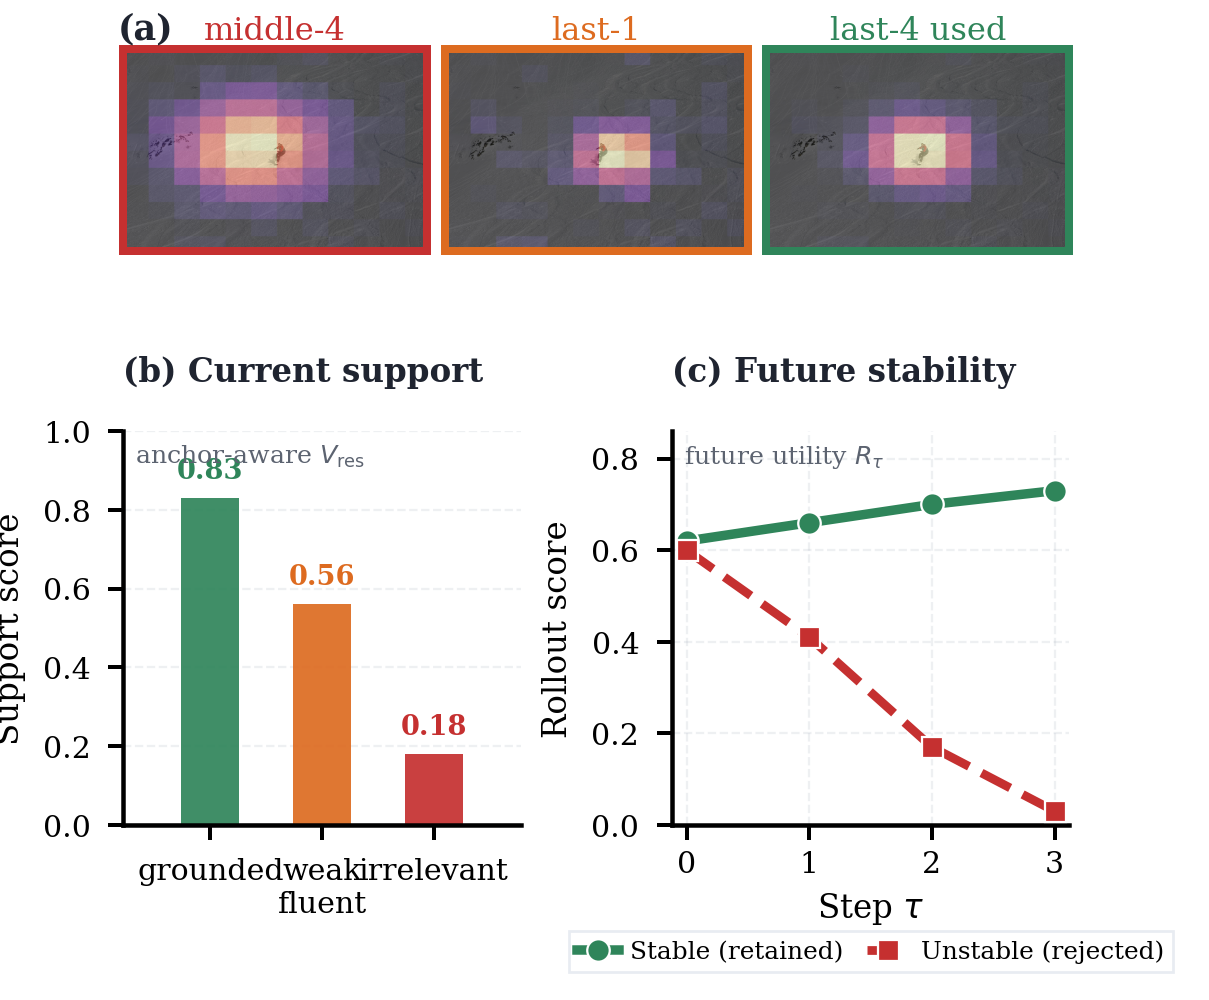
\includegraphics[width=\columnwidth]{figure4.png}
    \caption{Design evidence for CHORD. Top: decoder-to-vision heatmaps under three layer-selection choices, showing why CHORD uses the `last-4' window. Bottom-left: representative current-support scores for competing candidates at the admission step. Bottom-right: representative rollout utility traces showing how future arbitration separates a stable continuation from a text-dominated branch.}
    \Description{A single-column figure with a top row of three attention heatmaps and a bottom row of two compact charts. The heatmaps compare middle-4, last-1, and last-4 layer windows. The lower-left chart shows current support values for three candidate types. The lower-right chart shows rollout utility curves for a stable grounded branch and an unstable text-dominated branch.}
    \label{fig:design_evidence}
\end{figure}

\Fref{fig:qualitative_cases} combines three trace-backed POPE cases with one hard-negative decision case so that affirmative and negative queries can be compared under a consistent evidence template without overstating token-level trace availability.

\begin{figure}[t]
    \centering
    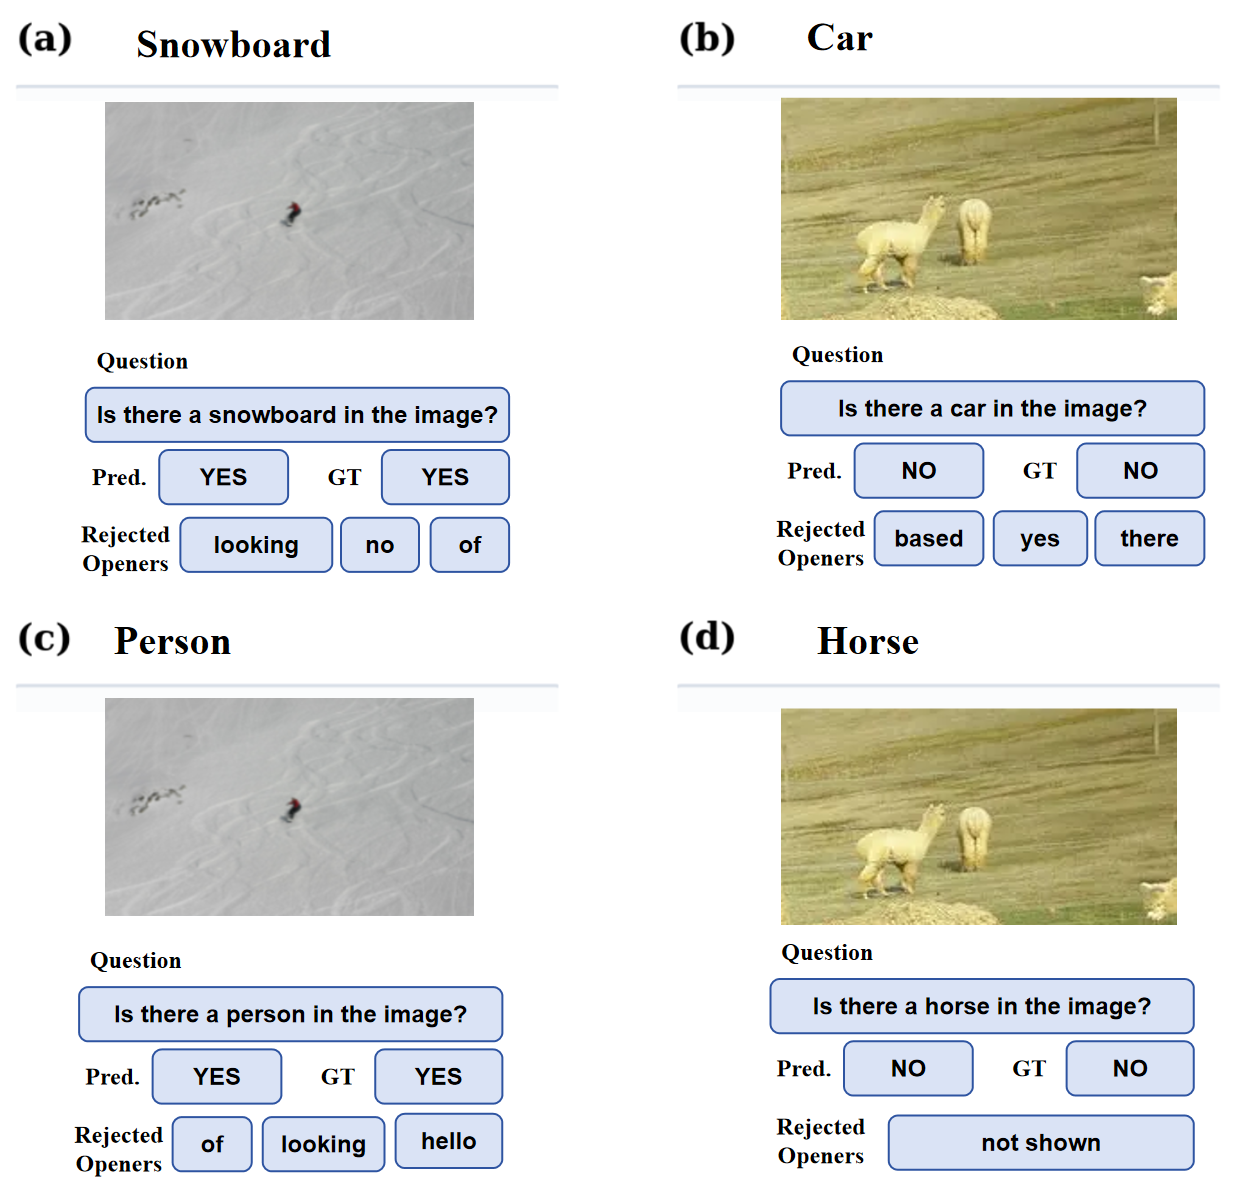
\includegraphics[width=\columnwidth,trim=12 12 12 12,clip]{figure5.png}
    \caption{Trace-backed qualitative evidence on four POPE-style cases. Panels (a)--(c) expose real rejected opener candidates suppressed during decoding, while panel (d) is reported as a hard-negative decision case without token-level trace annotation. Together they show how CHORD preserves grounded admissions and blocks weakly grounded continuations.}
    \Description{A single-column qualitative figure arranged as four compact case panels. Each panel places a real COCO image on the left and a small structured annotation area on the right.}
    \label{fig:qualitative_cases}
\end{figure}

The four panels separate two kinds of qualitative evidence. The snowboard and person examples are affirmative cases in which CHORD preserves the correct \texttt{yes} answer while suppressing weaker explanation-first alternatives. The car example is a trace-backed negative query on the same snowy scene, showing that CHORD can reject an unsupported object even when the visual context remains rich enough to encourage generic continuation. The horse panel is a hard-negative final-decision case in which the scene contains alpacas rather than horses, so we report only the final prediction rather than implying token-level trace availability. Qualitatively, CHORD is most informative when the top-$k$ set contains both a grounded candidate and one or more linguistically strong but weakly grounded competitors; if the proposer misses the key object entirely, decode-time control has substantially less room to recover.

\subsection{Operating-Point Synthesis}
\label{sec:efficiency}

\Fref{fig:quantitative} summarizes the operating landscape from the measured tables without repeating the raw table layout. Panels (a,b) place baselines and CHORD variants on the Adversarial F1 versus ITL plane, which makes the latency-quality frontier explicit. Panels (c,d) re-express the same methods on the CHAIR$_S$ versus MMBench plane, with marker size indicating ITL, so sentence-level suppression, retained general ability, and decode cost can be read together.

\begin{figure*}[t]
    \centering
    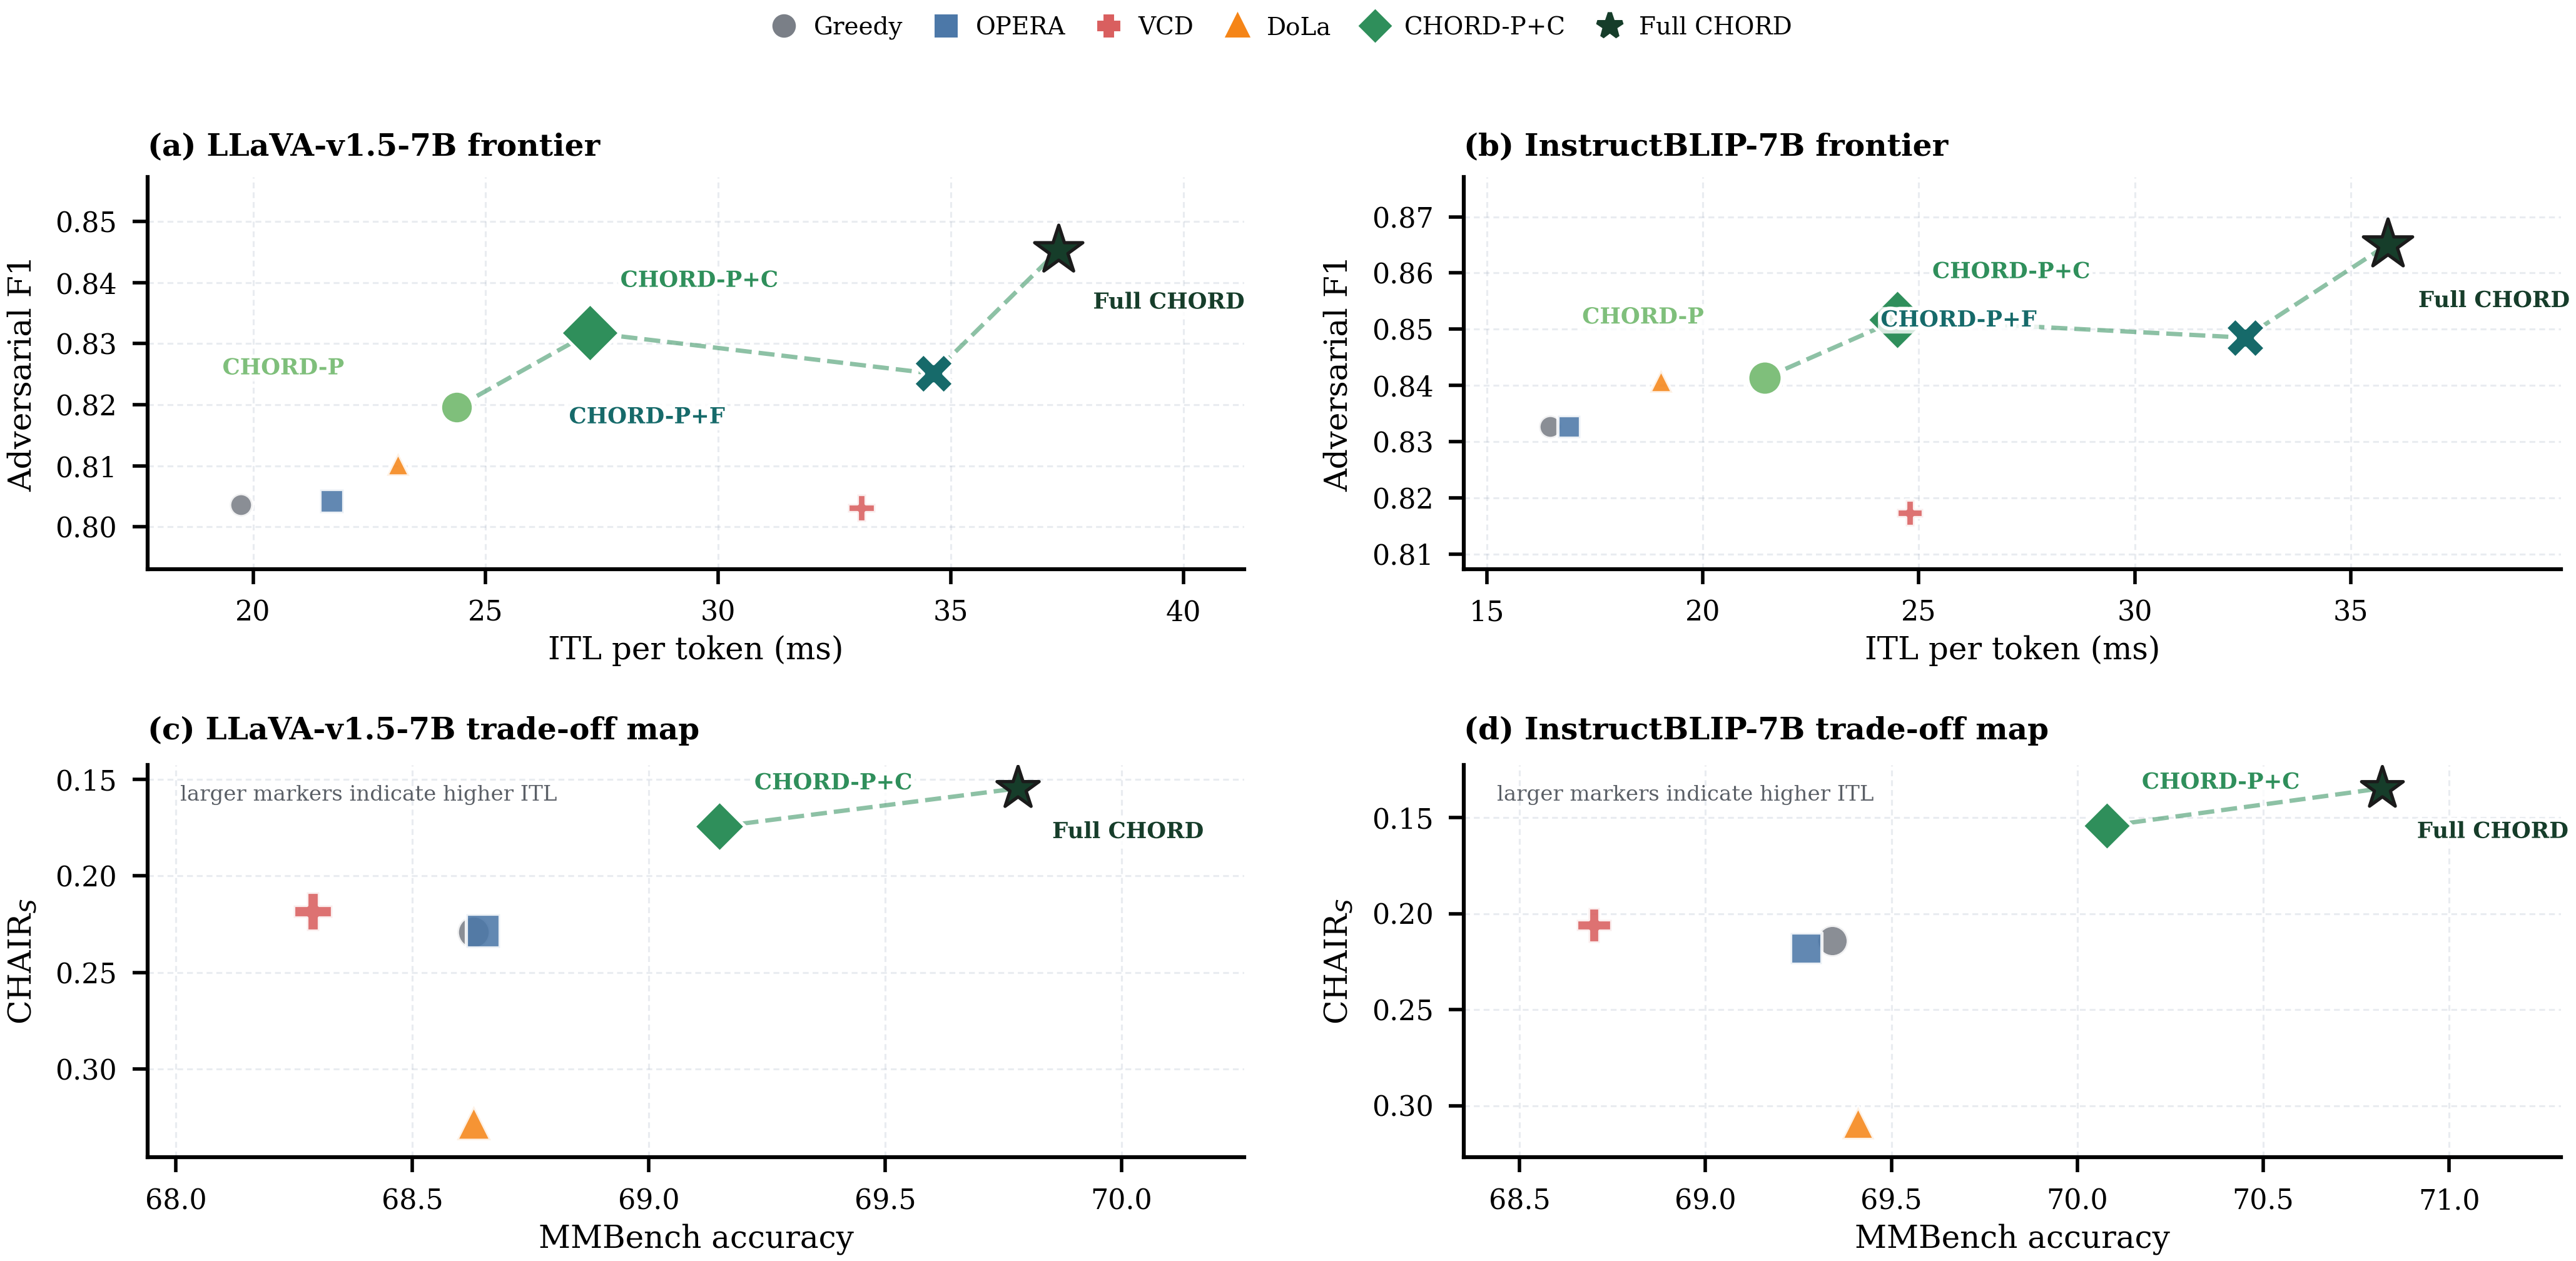
\includegraphics[width=\textwidth]{figure3.png}
    \caption{Quantitative synthesis of the main tables. (a,b) Adversarial F1 versus ITL. (c,d) CHAIR$_S$ versus MMBench with marker area proportional to ITL. The plots separate the efficiency-oriented \textit{CHORD-P+C} regime from quality-oriented Full CHORD.}
    \Description{A four-panel quantitative figure. The top row contains two scatter plots of adversarial F1 versus per-token latency for several decoding methods on LLaVA-v1.5-7B and InstructBLIP-7B. The bottom row contains two scatter plots of sentence-level CHAIR versus MMBench accuracy for the same methods, with larger markers indicating slower decoding.}
    \label{fig:quantitative}
\end{figure*}

The top row of \Fref{fig:quantitative} shows the same trend on both backbones: moving from Greedy or rollback-only baselines toward CHORD increases cost, but the CHORD family forms a coherent frontier rather than an arbitrary latency jump. \textit{Past+Current} remains near the efficient corner, whereas Full CHORD moves farther toward the best adversarial quality at higher ITL. The bottom row shows the second trade-off: the full configuration yields the largest sentence-level hallucination reduction while also retaining the best MMBench accuracy, whereas \textit{Past+Current} occupies the lower-cost middle ground. \Tref{tab:adv_breakdown} should be read alongside this figure: the adversarial gains are accompanied by higher precision, which is consistent with a more selective admission rule rather than a merely more conservative decoder.

\begin{table}[t]
\centering
\small
\setlength{\tabcolsep}{4pt}
    \caption{POPE Adversarial precision-recall breakdown for representative baselines and the two main CHORD operating points. \textit{CHORD-P+C} primarily improves robustness by raising precision without a large recall collapse, which is consistent with a better admission rule rather than a merely more conservative decoder.}
\label{tab:adv_breakdown}
\begin{tabular}{l l c c}
\toprule
\textbf{Model} & \textbf{Method} & Prec.~$\uparrow$ & Rec.~$\uparrow$ \\
\midrule
\multirow{5}{*}{LLaVA}
& Greedy        & 0.730 & \textbf{0.893} \\
& OPERA         & 0.732 & 0.893 \\
& VCD           & 0.748 & 0.867 \\
& CHORD-P+C     & 0.817 & 0.847 \\
& Full CHORD    & \textbf{0.842} & 0.849 \\
\midrule
\multirow{5}{*}{InstructBLIP}
& Greedy        & 0.772 & 0.858 \\
& OPERA         & 0.791 & \textbf{0.879} \\
& VCD           & 0.775 & 0.865 \\
& CHORD-P+C     & 0.841 & 0.863 \\
& Full CHORD    & \textbf{0.864} & 0.866 \\
\bottomrule
\end{tabular}
\end{table}

\subsection{Component Trade-off Within the CHORD Family}

To isolate the CHORD family itself, \Tref{tab:family_tradeoff} compares four representative variants across both backbones. This view clarifies how each component changes the decoder once the main cross-method comparison has established the overall performance pattern.

\begin{table}[t]
\centering
\scriptsize
\setlength{\tabcolsep}{3.0pt}
\caption{Trade-off within the CHORD family across both backbones. \textit{Past} is the lowest-latency correction, \textit{Past+Current} gives the best efficiency-quality compromise, and Full CHORD gives the strongest overall quality metrics.}
\label{tab:family_tradeoff}
\begin{tabular}{lcccccc}
\toprule
\multicolumn{7}{c}{\textbf{LLaVA-v1.5-7B}} \\
\textbf{Variant} & Avg. & Adv. & CH$_S$ & CH$_I$ & MMB & ITL \\
\midrule
Past      & 0.8583 & 0.8196 & 0.2042 & 0.1927 & 68.84 & \textbf{24.38} \\
Past+C    & 0.8647 & 0.8318 & 0.1745 & 0.1852 & 69.15 & 27.24 \\
Past+F    & 0.8625 & 0.8251 & 0.1794 & 0.1873 & 69.46 & 34.62 \\
Full      & \textbf{0.8752} & \textbf{0.8453} & \textbf{0.1548} & \textbf{0.1754} & \textbf{69.78} & 37.31 \\
\midrule
\multicolumn{7}{c}{\textbf{InstructBLIP-7B}} \\
\textbf{Variant} & Avg. & Adv. & CH$_S$ & CH$_I$ & MMB & ITL \\
\midrule
Past      & 0.8715 & 0.8413 & 0.1842 & 0.3158 & 69.64 & \textbf{21.43} \\
Past+C    & 0.8806 & 0.8517 & 0.1543 & 0.2946 & 70.08 & 24.51 \\
Past+F    & 0.8789 & 0.8485 & 0.1651 & 0.3042 & 70.43 & 32.55 \\
Full      & \textbf{0.8924} & \textbf{0.8651} & \textbf{0.1347} & \textbf{0.2795} & \textbf{70.82} & 35.86 \\
\bottomrule
\end{tabular}
\end{table}

Three conclusions follow from \Tref{tab:family_tradeoff}. First, rollback-based past protection already provides a strong correction at the lowest family latency. Second, adding current object resonance yields the strongest efficiency-quality compromise (\textit{Past+Current}, or \textit{CHORD-P+C}) on both backbones, even though the full configuration remains numerically best on the headline quality metrics. Third, future arbitration matters most for the quality-oriented regime: Full CHORD delivers the best family results, but also the largest latency increase.

\begin{table}[!b]
\centering
\scriptsize
\setlength{\tabcolsep}{3.5pt}
\caption{Deployment-oriented operating-point summary relative to Greedy. Negative $\Delta$CH values indicate hallucination reduction; positive $\Delta$ITL indicates extra latency. Higher $\Delta$Adv.\ F1/$\Delta$MMB are better, lower $\Delta$CH are better.}
\label{tab:operating_points}
\begin{tabular}{l l c c c c c}
\toprule
\textbf{Model} & \textbf{Regime} & $\Delta$Adv.\ F1~$\uparrow$ & $\Delta$CH$_S$~$\downarrow$ & $\Delta$CH$_I$~$\downarrow$ & $\Delta$MMB~$\uparrow$ & $\Delta$ITL~$\downarrow$ \\
\midrule
\multirow{2}{*}{LLaVA}
& P+C & +0.0282 & -0.0546 & -0.0194 & +0.52 & \textbf{+7.51} \\
& Full & \textbf{+0.0417} & \textbf{-0.0743} & \textbf{-0.0292} & \textbf{+1.15} & +17.58 \\
\midrule
\multirow{2}{*}{InstructBLIP}
& P+C & +0.0190 & -0.0597 & -0.0434 & +0.74 & \textbf{+8.04} \\
& Full & \textbf{+0.0324} & \textbf{-0.0793} & \textbf{-0.0585} & \textbf{+1.48} & +19.39 \\
\bottomrule
\end{tabular}
\end{table}

\Tref{tab:operating_points} summarizes the deployment trade-off. Across both backbones, \textit{Past+Current} (\textit{CHORD-P+C}) gives the best discriminative gain per added latency. Full CHORD provides stronger sentence-level suppression and slightly better retained benchmark accuracy, but at higher cost. We therefore present the two variants as complementary operating regimes rather than forcing a single universal default.

Taken together, \Tref{tab:family_tradeoff} and \Tref{tab:operating_points} sharpen the practical interpretation of CHORD. The family view shows that each added signal moves the decoder along a predictable axis rather than producing unstable metric swings: past protection provides the low-cost correction floor, current support yields the strongest marginal discriminative gain, and future arbitration mainly contributes additional robustness for longer open-ended outputs. This regularity is relevant for deployment because it allows the operating regime to be selected by latency budget and answer style without retuning the entire controller for each use case. Viewed this way, CHORD is better understood as a small family of controllable inference policies than as a single fixed decoding heuristic.

This operating-point reading also motivates reporting POPE, CHAIR, MMBench, and ITL jointly. A decoder that improves only one hallucination metric while eroding retained multimodal ability or imposing opaque latency cost is difficult to justify in practice. By contrast, the CHORD family traces a comparatively smooth frontier across both backbones, which suggests that its gains are not tied to a single benchmark artifact or isolated prompt style.

This cross-backbone consistency is an important empirical observation. Although LLaVA-1.5 and InstructBLIP differ in alignment recipe, visual backbone, and baseline latency, the same ranking reappears: \textit{Past+Current} (\textit{CHORD-P+C}) is the more efficient regime, while Full CHORD is the quality-oriented regime. This repeatability simplifies deployment-oriented interpretation, because the main decision is whether the target workload prioritizes lower latency or stronger open-ended suppression.

Methodologically, this pattern matches how CHORD decomposes admission control. The current term matters most when the candidate set already contains a clearly grounded option alongside linguistically plausible but weakly grounded distractors, whereas the future term matters more when an early weak admission would otherwise propagate across subsequent decoding steps. This is also the regime in which local support and short-horizon verification cease to be interchangeable. The tables therefore do more than rank methods: they show that the intended division between local support and short-horizon stability is observable at the benchmark level.

\section{Conclusion}
\label{sec:conclusion}

We presented \textbf{CHORD}, a training-free decoding framework that mitigates multimodal hallucination through bounded trajectory verification. By combining rollback-based historical protection, query-conditioned object resonance, and short-horizon rollout arbitration, CHORD turns token admission from a purely local choice into a grounded verifier-style decision.

Across LLaVA-1.5 and InstructBLIP, the experiments show a stable operating-point pattern: \textit{Past+Current} (\textit{CHORD-P+C}) is the more efficient choice when latency matters, while Full CHORD is stronger when longer free-form answers make early admission errors compound. This explicit quality-latency trade-off is the main practical conclusion of the study.

More broadly, these results suggest that decode-time hallucination control should be judged as an operating frontier rather than a single best number. The relevant question is how robustness, retained multimodal ability, and latency move together under realistic inference budgets, and CHORD provides one concrete template for that style of evaluation.

\noindent\textbf{Limitations \& Social Impact.}
CHORD improves grounding at additional test-time cost and remains bounded by visual evidence quality and the query-conditioned proposer. It reduces unstable continuation but does not guarantee factual correctness; in high-risk applications it should be treated only as a reliability aid.

\makeatletter
\@ACM@printacmreftrue
\makeatother
\clearpage
\bibliographystyle{ACM-Reference-Format}
\bibliography{sample-base}

\end{document}
